\documentclass[11pt]{article}
\usepackage{acl2015}
\usepackage{times}
\usepackage{url}
\usepackage{latexsym}
\usepackage{float}
\usepackage{booktabs}
\usepackage{tabularx}
\usepackage{array}
\usepackage{tikz}
\usetikzlibrary{arrows.meta,positioning}

\title{Detecting AI-generated text across different LLMs and domains\\Phase 1 proposal with SOTA analysis}
% https://www.overleaf.com/project/63440c16442dba647b52a1ae
\author{Oskar Szymanski (submitted by) \\
  01219844 \\
  {\scriptsize\tt oskar.szymanski2.stud@pw.edu.pl} \\\And
  Lukas Berner \\
  01219830 \\
  {\scriptsize\tt lukas\_berner.berner.stud@pw.edu.pl} \\ \And
  Bastian Kapfer \\
  01219842 \\
  {\scriptsize\tt bastian.kapfer.stud@pw.edu.pl} \\ \AND
  supervisor: Michał Gromadzki\\
  Warsaw University of Technology \\
  {\tt 01161435@pw.edu.pl}}

\date{}

\begin{document}
\maketitle

\section{Introduction}
Large language models (LLMs) produce fluent text in education, journalism, and online communication. Reliable detection of machine-generated text is therefore relevant to academic integrity and content provenance. However, high in-domain accuracy does not guarantee generalization: a detector may fail on an unseen generator, writing domain, prompt, or paraphrase. Watermarking offers a complementary approach by embedding a statistical signal during generation, but its detection depends on the watermark surviving later edits.

We propose a controlled comparison of (i) supervised classification, (ii) zero-shot statistical detection, and (iii) watermark detection. The central questions are whether detection transfers to unseen language models and domains, and how watermarking changes detection under controlled generation settings. We report area under the receiver operating characteristic curve (AUROC), the F1 score (harmonic mean of precision and recall), and true-positive rate (TPR) at a validation-calibrated false-positive rate (FPR). We also report the observed FPR on the held-out test set; it is not assumed to equal the validation target.

\section{State of the Art}
\label{sec:sota}
Supervised detectors learn from labelled examples and may overfit to the generators, domains, or prompts represented in training. Zero-shot detectors instead use token probabilities, ranks, entropy, or model comparisons without labelled target examples, although they may require access to reference language models. Watermark methods embed a keyed statistical signal during generation; their reliability depends on text length and resistance to edits. The tables below compare 17 representative studies from the state of the art. Each result is tied to the dataset, split, and operating point stated in its row (``split not stated'' where the paper gives none); scores are not directly comparable across papers.

\subsection{Supervised detection}
\begin{table*}[!t]
\centering\scriptsize
\begin{tabularx}{\textwidth}{>{\raggedright\arraybackslash}p{.15\textwidth} >{\raggedright\arraybackslash}p{.23\textwidth} >{\raggedright\arraybackslash}p{.36\textwidth} >{\raggedright\arraybackslash}X}
\toprule
\textbf{Study} & \textbf{Method} & \textbf{Dataset and split} & \textbf{Result}\\
\midrule
Zhou \& Wang \cite{zhou2024crossdomains} & RoBERTa-Ranker with similarity-based target adaptation. & ABSTRACT: human/GPT-4 abstracts; 1,000 labelled target texts for adaptation and 1,000 separate target texts for test. & F1: 78.3\% before and 85.8\% after adaptation.\\
Xia et al. \cite{xia2026explaining} & Fine-tuned DeBERTa-v3 and XLM-RoBERTa; analysis of 80 linguistic features. & arXiv, Amazon Reviews, CNN/DailyMail, ASQA; 3,000 sources per domain; 7 LLMs, 6 prompts; 50/17/33\% train/validation/test. Example transfer: train on arXiv, test on CNN/DailyMail. & Accuracy 0.57 (DeBERTa-v3-small, arXiv$\to$CNN/DailyMail, mean of seven generators); failures linked to shifts such as tense and pronoun use.\\
RoBERTa-base on DetectRL \cite{wu2024detectrl} & RoBERTa-base baseline (DetectRL is the benchmark, not a detector). & Domain-generalization task: train on one source domain, test on the other domains among arXiv, XSum, WritingPrompts, Yelp Reviews; aggregate over transfers. & F1: 83.00\%.\\
EAGLE \cite{bhattacharjee2024eagle} & RoBERTa with adversarial and contrastive learning. & TuringBench; train on five source generators, test on held-out GPT-3; mean over three seeds. & AUROC: 0.983 (preprint).\\
Ghostbuster \cite{verma2024ghostbuster} & Structured search over weaker-LM probability features, then a linear classifier; no target-model probabilities needed. & Student essays, creative writing, news; trained on two domains and tested on the held-out third; split not stated. & F1: 97.0\% averaged out-of-domain (99.0\% in-domain).\\
MAGE \cite{li2024mage} & Longformer in a multi-domain benchmark. & Testbed 6: leave one of ten source datasets out of training and test on the held-out dataset. & AUROC: 0.93; average recall: 68.4\%.\\
Easy2Hard \cite{wu2025easy2hard} & Auxiliary supervisor; RADAR and RADAR-E variants. & Essay, paragraph level; train on GPT4All and human text, test on Claude target examples. & TPR at 1\% FPR: 42.4\% / 55.9\% for RADAR / RADAR-E.\\
\bottomrule
\end{tabularx}
\caption{Supervised detectors and benchmark baselines.}
\label{tab:supervised}
\end{table*}

Zhou and Wang use labelled target examples, so their result measures adaptation rather than zero-shot generalization. DetectRL is a benchmark; its 83.00\% result belongs to the RoBERTa-base baseline. Ghostbuster reaches 99.0 F1 when trained and tested on the same domain but 97.0 F1 on held-out domains, which is the relevant figure for generalization. Xia et al.\ analyze transfer across prompt, model, and domain shifts rather than proposing a new detector.

\subsection{Zero-shot detection}
Zero-shot methods do not train on labelled target examples, but may require access to reference language models. Binoculars compares observer and performer models; DivScore uses domain knowledge distillation without labelled detector examples.

\begin{table*}[!t]
\centering\scriptsize
\begin{tabularx}{\textwidth}{>{\raggedright\arraybackslash}p{.15\textwidth} >{\raggedright\arraybackslash}p{.23\textwidth} >{\raggedright\arraybackslash}p{.36\textwidth} >{\raggedright\arraybackslash}X}
\toprule
\textbf{Study} & \textbf{Method} & \textbf{Dataset and split} & \textbf{Result}\\
\midrule
DetectLLM \cite{su-etal-2023-detectllm} & Log-likelihood log-rank ratio (LRR; no perturbation) and normalized perturbed log-rank (NPR; with perturbation). & XSum, SQuAD, WritingPrompts; 300 human and 300 machine texts per set; seven source LLMs (1.5--20B parameters); no detector training; split not stated. & AUROC, mean of seven LLMs (XSum/SQuAD/WritingPrompts): LRR 86.0/89.2/96.3\%; NPR 93.7/87.0/97.2\%.\\
Binoculars \cite{pmlr-v235-hans24a} & Cross-perplexity between an observer and a performer LLM (Falcon-7B pair). & ChatGPT-generated texts from the Ghostbuster News, Creative Writing, and Student Essay datasets; no detector training, so no train/test split. & TPR at 0.01\% FPR: 94.9/93.5/97.6\% (News/Creative Writing/Student Essay).\\
Tufts et al. \cite{tufts-etal-2025-practical} & Evaluation of four zero-shot (Fast-DetectGPT, PHD, LogRank, Binoculars) and three trained detectors under unseen tasks and prompting attacks. & Seven tasks (question answering, summarization, dialogue, code, abstracts, peer reviews, translation); per task 500 human texts and 400 machine texts from four LLMs; three tasks also in Spanish, French, Chinese; evaluation only. & Pooled over tasks and LLMs, TPR at 1\% FPR: Binoculars 0.58, Fast-DetectGPT 0.49, trained RADAR 0.05; AUROC 0.85/0.84/0.60; 0 in some task--LLM cells.\\
DivScore \cite{chen-etal-2025-divscore} & Normalized entropy with domain knowledge distillation (LoRA fine-tuning on LLM-written domain text; no labelled detection data). & MIMIC-IV-Note, PubMedQA, Open Australia Legal Corpus (OALC), LawStack; 1,000 human and 1,000 LLM texts per dataset and source LLM (GPT-4o, o3-mini, DeepSeek-V3, DeepSeek-R1); evaluation only. & Versus Binoculars: $+14.4$ AUROC points and $+64.0$ TPR points at 0.1\% FPR (mean over 4 datasets $\times$ 4 LLMs).\\
LLM-as-detector \cite{yuan2026crossgeneration} & 15 LLMs used as both generators and prompted detectors; cross-generation evaluation. & 1,000 human texts sampled from M4GT-Bench \cite{wang2024m4gt} plus 15,000 generated texts (1,000 per generator); 225 generator--detector pairs; evaluation only, no training split. & Mean F1: 69.5\%; accuracy: 76.5\% (SD 31.7/19.6 pp; preprint).\\
\bottomrule
\end{tabularx}
\caption{Zero-shot detection and evaluation studies. SD: standard deviation; pp: percentage points; LoRA: low-rank adaptation.}
\label{tab:zeroshot}
\end{table*}

Tufts et al.\ show that performance can collapse under task shift and rewriting, and that AUROC alone hides poor TPR at low FPR. DivScore is zero-shot with respect to labelled detection data, not training-free, and its gains are measured against Binoculars. Yuan et al.\ is a preprint, so its cross-generation results remain provisional.

\subsection{Watermarking and robustness}
Kirchenbauer et al.'s green-list watermark (KGW, after the initials of the first three authors) uses a secret key to select preferred tokens and slightly raises their logits during generation; detection tests whether green-token frequency is unusually high. Distortion-free schemes sample from the original model distribution using a key sequence. Both approaches can be weakened by paraphrasing.

\begin{table*}[!t]
\centering\scriptsize
\begin{tabularx}{\textwidth}{>{\raggedright\arraybackslash}p{.15\textwidth} >{\raggedright\arraybackslash}p{.23\textwidth} >{\raggedright\arraybackslash}p{.36\textwidth} >{\raggedright\arraybackslash}X}
\toprule
\textbf{Study} & \textbf{Method} & \textbf{Dataset and split} & \textbf{Result}\\
\midrule
Kirchenbauer et al. \cite{kirchenbauer2023watermark} & KGW green-list; logit bias and z-score detection. & C4 news-like prompts (split not stated); OPT-1.3B at 200 tokens; additional 30\% random token-replacement attack. & TPR: 98.4\% at z=4 with no observed false positives; AUROC: 0.954 after 30\% replacement.\\
Kuditipudi et al. \cite{kuditipudi2024distortionfree} & Distortion-free keyed sampling from the original model distribution. & OPT-1.3B/LLaMA-7B on C4 (split not stated); Alpaca-7B case study; random substitutions, insertions, and deletions. & Detectable from 35 tokens at $p\leq0.01$ after 40--50\% edits; about 25\% of Alpaca-7B answers detectable.\\
Dathathri et al. \cite{dathathri2024scalable} & SynthID-Text tournament sampling, including a non-distorting mode. & ELI5: 1,500 prompts in the distortionary test; 10,000 prompts in each non-distortionary development/test split; Gemma 2B/7B, Mistral 7B. & Higher TPR at 1\% FPR than Gumbel sampling (values only in figures); no significant change in user ratings over about 20 million live Gemini responses; 0.57\% added latency.\\
Krishna et al. \cite{krishna2023paraphrasing} & DIPPER paraphrase attack and retrieval defence. & WikiText-103 validation-split prompts and LFQA (3,000 each; LFQA has no standard split); GPT2-XL watermark; strongest paraphrase ($L=60$, $O=60$). & At 1\% FPR the watermark drops from 100\% to 57.2\% and DetectGPT from 70.3\% to 4.6\%; retrieval detects 97.8\% of paraphrases (80.4\% with 15 million stored generations).\\
Kirchenbauer et al. \cite{kirchenbauer2024reliability} & Improved KGW pipeline; sliding-window detection of watermarked spans. & C4 and LFQA (splits not stated); LLaMA-7B/Vicuna; GPT-3.5/DIPPER paraphrases and volunteer human rewrites. & Machine-paraphrase AUROC $>0.85$ at 200 tokens and $>0.9$ at 600; human rewrites detectable after about 800 tokens at $10^{-5}$ FPR.\\
\bottomrule
\end{tabularx}
\caption{Watermark methods and adversarial evaluations. C4: Colossal Clean Crawled Corpus; ELI5: Explain Like I'm Five (Reddit question answering); LFQA: long-form question answering; OPT: Open Pre-trained Transformer; LLaMA: Large Language Model Meta AI; DIPPER: Discourse Paraphraser; $L$, $O$: its lexical and order diversity settings.}
\label{tab:watermark}
\end{table*}

The literature indicates that watermarks can be detectable in unmodified outputs yet degrade under paraphrasing. We will therefore evaluate KGW only on controlled texts whose generation metadata records whether watermarking was enabled.

\section{Datasets and status}
All labels refer to text origin (human or machine); model and watermark condition are retained as secondary metadata. We will not use a dataset marked RESTRICTED. Public datasets are READY; our controlled generation collection is TO COLLECT.

\noindent\textbf{RAID} \cite{dugan2024raid} (\textbf{READY}): approximately 6.3 million texts, including about 5.4 million labelled training examples; 8 domains, 11 generators, 4 decoding strategies, and 11 attacks. Labels distinguish human text from generator outputs. The human class is about 3\%, so we will use documented balanced subsets for training while retaining condition-specific evaluation results. Distributed via Hugging Face (\texttt{liamdugan/raid}); dataset licence: MIT.

\noindent\textbf{WritingPrompts} \cite{fan2018hierarchical} (\textbf{READY}): 303,358 human stories (272,600 train; 15,620 validation; 15,138 test; mean length about 735 words). All records are human-written and are used as human examples and prompt sources, not as a mixed human/machine benchmark. The cited Hugging Face mirror lists MIT metadata; because the content originates from Reddit, we will retain source attribution and check applicable source/platform terms before redistribution. Obtained from \texttt{euclaise/writingprompts}.

\noindent\textbf{HC3-English} \cite{guo2023hc3} (\textbf{READY}): 24,322 questions with 58,546 human and 26,903 ChatGPT answers across Reddit ELI5 (Explain Like I'm Five), open QA, Wikipedia/CS, medicine, and finance. Labels distinguish human from ChatGPT answers; answer-level balance is about 69\% human and 31\% machine. The Hugging Face dataset card lists CC BY-SA 4.0, while stricter source-dataset terms may apply. Obtained from \texttt{Hello-SimpleAI/HC3}.

\noindent\textbf{Controlled generations} (\textbf{TO COLLECT}): 7,000 texts: 1,000 matched WritingPrompts prompt/story pairs plus 6,000 generated texts (1,000 prompts $\times$ 3 models $\times$ 2 settings; one human story per prompt). Models: Llama 3.1 8B Instruct and Qwen2.5 7B Instruct, which are not among RAID's generators, and Mistral 7B Instruct, whose model family RAID covers and which therefore serves as a control; settings: KGW watermark on/off with matched decoding settings and a target length of about 500 words. Labels and model/watermark metadata are assigned automatically at generation time. Class balance is 1,000 human to 6,000 machine (1:6); balanced training subsets will be sampled, and results will also be reported by model and watermark condition. Oskar is responsible for collection by 8 November 2026; the team will spot-check outputs. Generated texts follow the respective Llama Community and Apache 2.0 model terms.

\section{Solution concept and experimental plan}
\paragraph{Success deliverables.}
(1) A reproducible benchmark with documented labels, grouped splits, and balanced training subsets. (2) Three working approaches: fine-tuned RoBERTa, a zero-shot detector (Binoculars), and a KGW watermark detector on controlled generations. (3) Evaluation tables, scripts, and error analysis for held-out generators, domains, and watermark settings.

\begin{figure}[t]
\centering
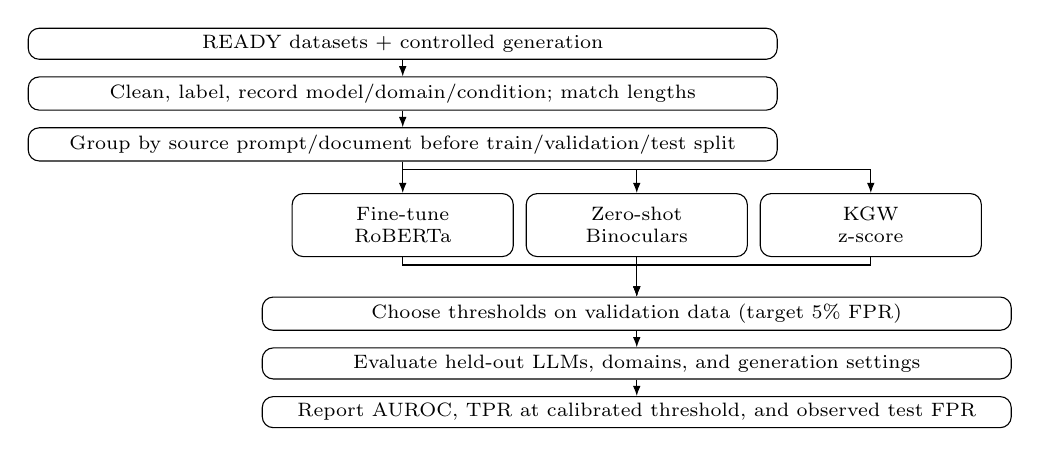
\begin{tikzpicture}[node distance=2.1mm,
  box/.style={draw,rounded corners,align=center,font=\scriptsize,text width=.77\columnwidth,inner sep=2.5pt},
  method/.style={draw,rounded corners,align=center,font=\scriptsize,text width=.22\columnwidth,minimum height=8mm,inner sep=2pt},
  arr/.style={-{Latex[length=1.3mm]},thin}]
\node[box] (data) {READY datasets + controlled generation};
\node[box,below=of data] (prep) {Clean, label, record model/domain/condition; match lengths};
\node[box,below=of prep] (split) {Group by source prompt/document before train/validation/test split};
\node[method,below=4mm of split] (sup) {Fine-tune\\RoBERTa};
\node[method,right=1.5mm of sup] (zero) {Zero-shot\\Binoculars};
\node[method,right=1.5mm of zero] (wm) {KGW\\z-score};
\node[box,below=5mm of zero] (cal) {Choose thresholds on validation data (target 5\% FPR)};
\node[box,below=of cal] (test) {Evaluate held-out LLMs, domains, and generation settings};
\node[box,below=of test] (metrics) {Report AUROC, TPR at calibrated threshold, and observed test FPR};
\draw[arr] (data)--(prep); \draw[arr] (prep)--(split);
\draw[arr] (split.south)--++(0,-1mm)-|(sup.north);
\draw[arr] (split.south)--++(0,-1mm)-|(zero.north);
\draw[arr] (split.south)--++(0,-1mm)-|(wm.north);
\draw[arr] (sup.south)--++(0,-1mm)-|(cal.north);
\draw[arr] (zero)--(cal); \draw[arr] (wm.south)--++(0,-1mm)-|(cal.north);
\draw[arr] (cal)--(test); \draw[arr] (test)--(metrics);
\end{tikzpicture}
\caption{Planned experimental pipeline. The test set is not used for threshold selection.}
\label{fig:pipeline}
\end{figure}

All texts derived from the same prompt or source document will remain in one split to prevent leakage. For leave-one-generator-out and leave-one-domain-out experiments, the held-out source will be excluded from detector training. Thresholds will be selected on validation data only (target FPR 5\%); final test results will include the observed FPR. We will report AUROC, TPR at the selected threshold, and observed FPR for each held-out condition. For the watermark detector, KGW-enabled texts are the positives; human texts and unwatermarked machine texts generated from the same prompts are the negatives.

\begin{table}[t]
\centering\scriptsize
\begin{tabularx}{\columnwidth}{@{}p{.25\columnwidth} X p{.13\columnwidth}@{}}
\toprule
\textbf{Week} & \textbf{Task / output} & \textbf{Owner}\\
\midrule
2--8 Nov & Generate and spot-check controlled texts & O\\
9--15 Nov & Prepare data; create grouped splits; implement baselines & B, L, O\\
16--22 Nov & Baseline evaluation and threshold calibration & B, L, O\\
23--29 Nov & Leave-one-LLM-out evaluation & B, L\\
30 Nov--6 Dec & Leave-one-domain-out evaluation & B, L\\
7--13 Dec & Watermark and generation-setting tests & B, L, O\\
14--20 Dec & HC3 external evaluation; repeat comparisons & B, L, O\\
21--27 Dec & Error analysis; freeze results by 23 Dec & B, L, O\\
28 Dec--3 Jan & Winter-break buffer & --\\
4--10 Jan & Reproducibility checks and report consolidation & B, L, O\\
11--13 Jan & Final edits and submission & All\\
\bottomrule
\end{tabularx}
\caption{Work plan. B: Bastian (supervised); L: Lukas (zero-shot); O: Oskar (data/watermarking).}
\label{tab:plan}
\end{table}

\section{Data statement}
We use RAID, WritingPrompts, HC3, and texts generated for this project. RAID is distributed under MIT terms; the cited WritingPrompts mirror lists MIT metadata, subject to source/platform terms for Reddit-origin content. HC3 is listed as CC BY-SA 4.0, with stricter source terms taking precedence where applicable. Generated texts are subject to the respective model licences. HC3 and Reddit-derived texts may contain personal or sensitive information; we will not attempt author identification and will keep project copies on secure storage with access limited to team members. We will share generated texts and prompt identifiers, but not redistribute original human texts.

\section{Contribution table}

\begin{table}[H]
  \centering
  \small
  \begin{tabularx}{\columnwidth}{
      >{\raggedright\arraybackslash}X
      >{\raggedright\arraybackslash}p{0.22\columnwidth}
      r
  }
    \toprule
    Task & Member & Hours \\
    \midrule
    Research & Bastian, Lukas, Oskar & 4 \\
    Introduction &  Bastian, Lukas, Oskar & 0.5 \\
    State of the art: supervised detectors & Bastian & 7 \\
    State of the art: zero-shot detectors & Lukas & 10 \\
    State of the art: watermark-based detection & Oskar & 12 \\
    Datasets and their status & Oskar & 5 \\
    Solution concept and experimental plan & Bastian & 1 \\
    Declaration of LLM use & Bastian & 0.5 \\
    \midrule
    \multicolumn{2}{l}{Total} & 40 \\
    \bottomrule
  \end{tabularx}
  \caption{Contribution of each team member and workload in hours.}
  \label{tab:contribution_table}
\end{table}

\section{Declaration of LLM use}
OpenAI ChatGPT and Anthropic Claude were used to support literature exploration, to locate and read the cited papers, to explain papers and evaluation metrics, to check reported numbers and dataset descriptions against the sources, to revise report text, and to draft LaTeX tables, figures, and BibTeX entries. The team is responsible for the submitted work and will verify references, factual claims, and numerical results against the cited sources. In later phases, any use for coding, debugging, or result interpretation will be documented together with verification steps.

\bibliographystyle{acl}
\bibliography{references}
\end{document}